\documentclass[twocolumn]{article}
\usepackage{latex8}
\usepackage{graphicx}

\begin{document}
\title{Reconstructino of Suspended Sediment using Artificial Intelligence}
\author{Dominic Mutzhas}
\maketitle

\begin{abstract} 

\end{abstract} 


\section{Introduction}
Accurate suspended sediment modeling is needed for a variety of reasons. One example is the planning of hydraulic river structures like water reservoirs, where the slowing of the water leads to a deposition of suspended sediment, and eventually to complete aggradation. \\
Since the interaction between hydraulic structures and the environment is very complex, any available data in that flied is important, and supended sediment data can be helpful in evaluating the impact of hydraulic structures on ecosystems.
Predicting these much needed values turns out to be a difficult problem, since Erosion and sediment transport are very physically complex phenomena. Thus the accuracy of physical models is also limited, since The large number of [obscure] parameters involved, requires many assumptions and simplifications to be made.
This difficulty has lead to the development of data driven methods,where the rivers suspended sediment dynamic is approximated with a model which is built directly from the data. One big advantage with these methods is that the data implicitely represents the physical phenomena, and thus allow modeling, without requiring any knowlege about the actualy physical theory. 
A very common yet very simple version of a data driven Models is the classic power function SRC: 
 


As the machine learning(ML) revolution progresses, more and more scientific disciplines are trying to take advantage of it's strenghts in handling complex and non-linear problems. As such it has also found it's way into the field of water management in the form of artificial neural networks (ANN), especially for the prediction of Flow and suspended Sediment.


\section{Background} 
Smartphones are increasingly being used to store personal information as well as to access sensitive data from the Internet and the cloud. Establishment of the identity of a user requesting information from smartphones is a prerequisite for  secure systems in such scenarios. In the past, keystroke-based user identification has been successfully deployed on production-level mobile devices to mitigate the risks associated with naive username/password based authentication. However, these approaches have two major limitations: they are not applicable to services where authentication occurs outside the domain of the mobile
device such as web-based services; and they often overly tax the limited computational capabilities of mobile devices. In this paper, we propose a protocol for keystroke dynamics analysis which allows web-based applications to make use of remote attestation and\cite{nauman2011using} delegated keystroke analysis. The end result is an efficient keystroke-based user identification mechanism that strengthens traditional password protected services
while mitigating the risks of user profiling by \cite{se-cs-collab:nauman10}collaborating malicious web
services. We present a prototype implementation of our protocol using
the popular Android operating system for smartphones.\cite{seo2011user}

\subsection{Some Related Work} 
Establishment of the identity of a user requesting information from smartphones is a prerequisite for  secure systems in such scenarios. In the past, keystroke-based user identification has been successfully deployed on production-level mobile devices to mitigate the risks associated with naive username/password based authentication. However, these approaches have two major limitations: they are not applicable to services where authentication occurs outside the domain of the mobile
device such as web-based services; and they often overly tax the limited computational capabilities of mobile devices. In this paper, we propose a protocol for keystroke dynamics analysis which allows web-based applications to make use of remote attestation and delegated keystroke analysis.

\section{Conclusions}

\begin{figure}
	\centering
	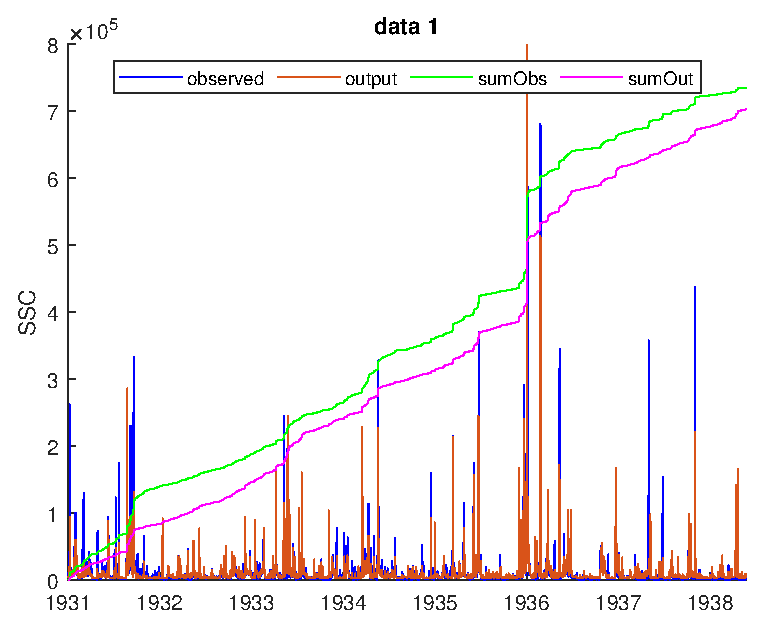
\includegraphics{epsFig}
	\caption{Insert caption}
\end{figure}

In the past, keystroke-based user identification has been successfully deployed on production-level mobile devices to mitigate the risks associated with naive username/password based authentication. However, these approaches have two major limitations: they are not applicable to services where authentication occurs outside the domain of the mobile
device such as web-based services.


\input{subfile_0}

% -------------------------------------------------------------------
% add bibliography-related commands here 
\bibliographystyle{IEEEtran}
\bibliography{bibfile_Thesis}   
\end{document}